\section{字符串}

\subsection{Hash}

\begin{lstlisting}[language=C++]
constexpr int P = 131, mod1 = 998244353, mod2 = 1e9 + 7;
struct Hash {
    vector<int> p1, h1;
    vector<int> p2, h2;
    Hash() {}
    Hash(string s) {
        init(s);
    }
    void init(string s) {
        int n = s.size();
        p1.assign(n, 1);
        h1.assign(n, 0);
        // p2.assign(n, 1);
        // h2.assign(n, 0);

        for (int i = 1; i < n; i++) {
            p1[i] = p1[i - 1] * P % mod1;
            h1[i] = (h1[i - 1] * P % mod1 + s[i]) % mod1;

            // p2[i] = p2[i - 1] * P % mod2;
            // h2[i] = (h2[i - 1] * P % mod2 + s[i]) % mod2;
        }
    }
    int substr_hash1(int l, int r) {
        int hash1 = ((h1[r] - h1[l - 1] * p1[r - l + 1] % mod1) % mod1 + mod1) % mod1;
        return hash1;
    }
    int substr_hash2(int l, int r) {
        int hash2 = ((h2[r] - h2[l - 1] * p2[r - l + 1] % mod2) % mod2 + mod2) % mod2;
        return hash2;
    }
};
\end{lstlisting}

\subsection{KMP}

前缀函数 $\pi[i]$：前 $i$ 个字符中，能够匹配的最长真前缀与真后缀。

若当前位置失配，则（在 $s[0\dots \pi[j]-1]$ 中）寻找次长的相匹配的前后缀。

转移：$j^{(k)}=\pi[j^{(k-1)}-1]$ (下标从0开始)。

KMP：查找 s 在 t 中的所有出现，对 s+'\#'+t 求前缀函数。

\begin{lstlisting}[language = C++]
int n = str.size(), m = text.size();
s = str+'#'+text;
// 求前缀函数
for (int i = 1; i < n; i++) {
    int j = pi[i - 1];
    while (j > 0 && s[i] != s[j]) j = pi[j - 1];
    if (s[i] == s[j]) j++;
    pi[i] = j;
}
// 统计答案
vector<int> v;
for(int i = n+1; i < s.size(); i++)
    if(pi[i] == n) v.push_back(i-2*n);
\end{lstlisting}

\begin{lstlisting}[language = C++]
// 1-based kmp，nxt[i] = i失配应跳转的下标 = pre[i - 1]的最长border + 1
vector<int> kmp(string s) {
    int n = s.size() - 1;
    vector<int> nxt(n + 2, 1);
    for (int i = 2, j = 1; i <= n; i++) {
        while (j > 1 && s[i] != s[j]) {
            j = nxt[j];
        }
        j += (s[i] == s[j]);
        nxt[i + 1] = j;
    }
    return nxt;
}
void solve() {
    string s1, s2;
    cin >> s1 >> s2;
    int n1 = s1.size(), n2 = s2.size();

    s1 = '0' + s1;
    s2 = '0' + s2;

    auto nxt = kmp(s2);
    for (int i = 1, j = 1; i <= n1; i++) {
        while (j > 1 && s1[i] != s2[j]) {
            j = nxt[j];
        }
        j += (s1[i] == s2[j]);
        if (j > n2) {
            cout << i - n2 + 1 << "\n";
            j = nxt[j];
        }
    }
    for (int i = 2; i <= n2 + 1; i++) {
        cout << nxt[i] - 1 << " \n"[i == n2 + 1];
    }
}
// by lyh
\end{lstlisting}

\subsection{AC 自动机}

$fail[u]$：状态 $u$ 的最长真后缀

$ch[u][i]$：字典图的边，若在字典树中不存在该边，则连向 $ch[fail[u]][i]$

\begin{lstlisting}[language = C++]
// 统计每一个模式串 $t_i$ 在文本串 $s$ 中出现的次数
struct AC_automation{
    int m, tot;
    
    struct node{
        int fail, val, id, ch[26];
        node(){
            fail = val = id = 0;
            memset(ch, 0, sizeof(ch));
        }
    }tr[N];
    
    AC_automation() {m = tot = 0;}
    // 构建字典树
    void insert(const string &t, int &idx){
        int p = 0;
        for(int i = 0; i < t.size(); i++){
            int &nxt = tr[p].ch[t[i]-'a'];
            if(nxt) p = nxt;
            else p = nxt = ++tot;
        }
        if(!tr[p].id) tr[p].id = ++m;
        idx = tr[p].id;
    }
    // 构建字典图
    void build(){
        queue<int> q;
        for(int i = 0; i < 26; i++)
            if(tr[0].ch[i]){
                q.push(tr[0].ch[i]);
                g[0].push_back(tr[0].ch[i]);
            }
        while(q.size()){
            int p = q.front();
            q.pop();
            for(int i = 0; i < 26; i++){
                int &nxt = tr[p].ch[i];
                if(nxt){
                    tr[nxt].fail = tr[tr[p].fail].ch[i];
                    g[tr[nxt].fail].push_back(nxt);
                    q.push(nxt);
                }
                else nxt = tr[tr[p].fail].ch[i];
            }
        }
    }
    // 匹配最长后缀并打标记
    void query(const string &s){
        int p = 0;
        for(int i = 0; i <= m; i++)
            tr[i].val = 0;
        for(int i = 0; i < s.size(); i++){
            p = tr[p].ch[s[i]-'a'];
            if(p) tr[p].val++;
        }
    }
    // dfs在fail树上做后缀和
    void dfs(int u){
        for(auto v: g[u]){
            dfs(v);
            tr[u].val += tr[v].val;
        }
        if(tr[u].id) ans[tr[u].id] = tr[u].val;
    }
};
\end{lstlisting}

ACAM 

\begin{lstlisting}[language=C++]
struct ACAM {
    static constexpr int ALPHABET_SIZE = 26;
    struct Node {
        int fail;
        array<int, ALPHABET_SIZE> ch;
        int len, cnt;
        Node() : fail{}, ch{}, len{}, cnt{} {}
    };
    int tot;
    vector<Node> t;
    ACAM() {
        init();
    }
    void init() {
        tot = 1;
        t.assign(1, Node());
    }
    int newNode() {
        tot++;
        t.emplace_back();
        return tot - 1;
    }
    void insert(string s) {
        int p = 0;
        for (int i = 0; i < s.size(); i++) {
            int c = s[i] - 'a';
            if (!t[p].ch[c]) {
                t[p].ch[c] = newNode();
            }
            p = t[p].ch[c];
        }
        t[p].len = s.size();
        t[p].cnt++;
    }
    void build() {
        queue<int> q;
        for (int c = 0; c < ALPHABET_SIZE; c++) {
            if (t[0].ch[c]) {
                q.push(t[0].ch[c]);
            }
        }
        while (!q.empty()) {
            auto u = q.front();
            q.pop();
            for (int c = 0; c < ALPHABET_SIZE; c++) {
                if (t[u].ch[c]) {
                    t[t[u].ch[c]].fail = t[t[u].fail].ch[c];
                    q.push(t[u].ch[c]);
                } else {
                    t[u].ch[c] = t[t[u].fail].ch[c];
                }
            }
        }
    }
    Node& operator[](const int &id) {
        return t[id];
    }
};
// by lyh
\end{lstlisting}

\subsection{SAM}

\begin{lstlisting}[language=C++]

struct SAM {
    static constexpr int ALPHABET_SIZE = 26;
    struct Node {
        int len = 0;
        int link = 0;
        array<int, ALPHABET_SIZE> ch;
        int siz = 0, rpos = -1;

    };
    vector<Node> t;
    int last;
    SAM() {
        init();
    }
    void init() {
        last = 1;
        t.assign(2, Node());
    }
    int newNode() {
        t.emplace_back();
        return t.size() - 1;
    }
    void extend(int c, int id) {
        int p = last, cur = newNode();
        t[cur].len = t[p].len + 1;
        for (; p && !t[p].ch[c]; p = t[p].link) {
            t[p].ch[c] = cur;
        }
        if (!p) {
            t[cur].link = 1;
        } else {
            int q = t[p].ch[c];
            if (t[q].len == t[p].len + 1) {
                t[cur].link = q;
            } else {
                int r = newNode();
                t[r].len = t[p].len + 1;
                t[r].link = t[q].link;
                t[r].ch = t[q].ch;
                t[cur].link = t[q].link = r;
                for (; p && t[p].ch[c] == q; p = t[p].link) {
                    t[p].ch[c] = r;
                }
                t[r].rpos = t[q].rpos;
            }
        }
        last = cur;
        t[cur].siz = 1;
        t[cur].rpos = id;
    }
    Node &operator[](const int &id) {
        return t[id];
    }
};
void build_rpos(int n, int tot) {
    vector<int> cnt(n + 1), order(tot + 1);
    for (int i = 2; i <= tot; i++) {
        cnt[sam[i].len]++;
    }
    for (int i = 1; i <= n; i++) {
        cnt[i] += cnt[i - 1];
    }
    for (int i = tot; i >= 1; i--) {
        order[cnt[sam[i].len]--] = i;
    }
    for (int i = tot; i >= 1; i--) {
        int u = order[i], p = sam[u].link;
        sam[p].siz += sam[u].siz;
        sam[p].rpos = max(sam[p].rpos, sam[u].rpos);
    }
}
vector<array<int, 2>> debug_adj[N];
void output(int u, int p) {
    cout << u << ": \n";
    for (auto [v, w] : debug_adj[u]) {
        cout << u << "-" << v << ": " << char(w + 'a') << "\n";
    }
    int l = sam.t[p].len + 1;
    int r = sam.t[u].len;
    for (int len = l; len <= r; len++) {
        cout << s.substr(sam.t[u].rpos - len + 1, len) << "\n";
    }
    cout << "\n";
    for (auto [v, w] : debug_adj[u]) {
        output(v, u);
    }
}
void debug(int n, int tot) {
    build_rpos(n, tot);
    for (int i = 2; i <= tot; i++) {
        int p = sam.t[i].link;
        int c = s[sam.t[i].rpos - sam.t[p].len - 1] - 'a';
        debug_adj[p].push_back({i, c});
    }
    output(1, 0);
}

s = '0' + s;
for (int i = 1; i <= n; i++) {
    sam.extend(s[i] - 'a', i);
}
\end{lstlisting}

\begin{figure}[htbp]
    \centering
    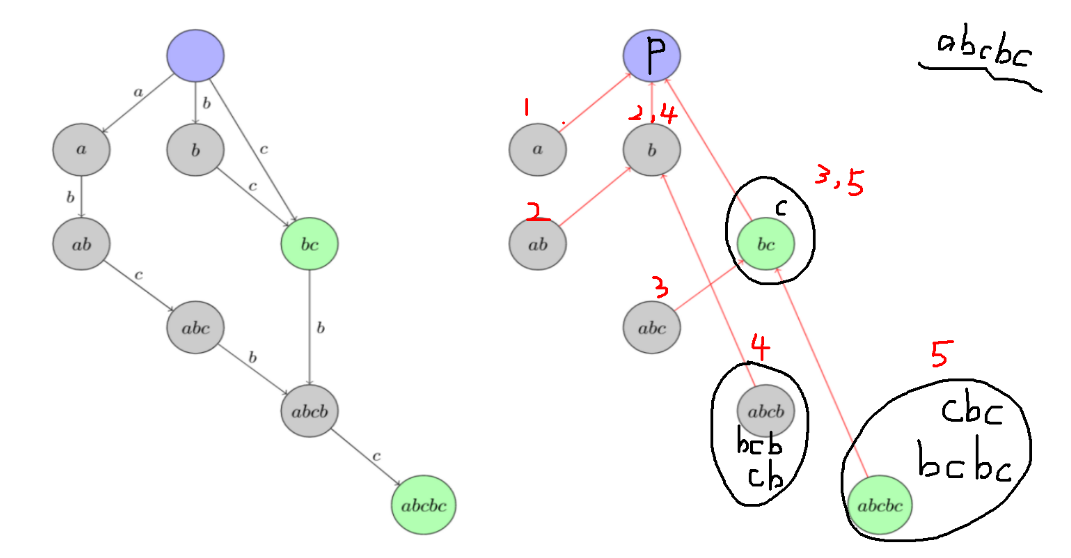
\includegraphics[scale=0.25]{lyh/SAM.png}
    \caption{SAM}
\end{figure}

\subsection{SA}

\begin{lstlisting}[language=C++]
s// 1-based
struct SA {
    int m = 127;
    int n;
    vector<int> sa, rk, height;
    SA(const string &s) {
        n = s.size() - 1;
        sa.resize(n + 1);
        rk.resize(n + 1);
        height.resize(n + 1);
        vector<int> cnt(m + 1);
        for (int i = 1; i <= n; i++) {
            cnt[rk[i] = s[i]]++;
        }
        for (int i = 1; i <= m; i++) {
            cnt[i] += cnt[i - 1];
        }
        for (int i = n; i >= 1; i--) {
            sa[cnt[rk[i]]--] = i;
        }
        vector<int> id(n + 1), oldrk;
        for (int w = 1, p; ; w <<= 1, m = p) {
            int cur = 0;
            for (int i = n - w + 1; i <= n; i++) {
                id[++cur] = i;
            }
            for (int i = 1; i <= n; i++) {
                if (sa[i] > w) {
                    id[++cur] = sa[i] - w;
                }
            }
            cnt.assign(m + 1, 0);
            for (int i = 1; i <= n; i++) {
                cnt[rk[i]]++;
            }
            for (int i = 1; i <= m; i++) {
                cnt[i] += cnt[i - 1];
            }
            for (int i = n; i >= 1; i--) {
                sa[cnt[rk[id[i]]]--] = id[i];
            }
            oldrk = rk;
            p = 0;
            for (int i = 1; i <= n; i++) {
                if (oldrk[sa[i]] == oldrk[sa[i - 1]] && 
                    oldrk[sa[i] + w] == oldrk[sa[i - 1] + w]) {
                    rk[sa[i]] = p;
                } else {
                    rk[sa[i]] = ++p;
                }
            }
            if (p == n) break;
        }
        for (int i = 1, j = 0; i <= n; i++) {
            if (rk[i] == 1) continue;
            if (j) j--;
            while (s[i + j] == s[sa[rk[i] - 1] + j]) {
                j++;
            }
            height[rk[i]] = j;
        }
    }
};

// 应用
int L = 2 * n, K = 20;
vector st(L + 1, vector<int>(K));
for (int i = 1; i <= L; i++) {
    st[i][0] = sa.height[i];
}
for (int j = 1; j < K; j++) {
    for (int i = 1; i + (1 << j) - 1 <= L; i++) {
        st[i][j] = min(st[i][j - 1], st[i + (1 << j - 1)][j - 1]);
    }
}
auto rmq = [&](int l, int r) {
    int k = __lg(r - l + 1);
    return min(st[l][k], st[r - (1 << k) + 1][k]);
};
auto lcp = [&](int i, int j) {
    if (i == j) {
        return n - i + 1;
    }
    int a = sa.rk[i];
    int b = sa.rk[j];
    if (a > b) {
        swap(a, b);
    }
    return rmq(a + 1, b);
};
auto lcs = [&](int i, int j) {
    if (i == j) {
        return i;
    }
    int a = sa.rk[2 * n + 1 - i];
    int b = sa.rk[2 * n + 1 - j];
    if (a > b) {
        swap(a, b);
    }
    return rmq(a + 1, b);
};
// by lyh
\end{lstlisting}

\subsection{SAIS}

\begin{lstlisting}[language=C++]
struct SA {
    vector<int> sa, rk, height;
    SA(const string &init) {
        int n = init.size() - 1;
        vector<int> s;
        for (int i = 1; i <= n; i++) {
            s.push_back(init[i]);
        }
        s.push_back(0);

        sa = SAIS(s, 128);
        rk.assign(n + 1, 0);
        height.assign(n + 1, 0);
        for (int i = 1; i <= n; i++) {
            sa[i]++;
            rk[sa[i]] = i;
        }
        for (int i = 1, j = 0; i <= n; i++) {
            if (rk[i] == 1) continue;
            if (j) j--;
            while (init[i + j] == init[sa[rk[i] - 1] + j]) {
                j++;
            }
            height[rk[i]] = j;
        }
    }
    bool is_LMS_char(const vector<bool> &type, int x) {
        return x >= 1 && type[x] == 1 && type[x - 1] == 0;
    }
    bool is_LMS_equal(const vector<int> &s, vector<bool> &type, int x, int y) {
        do {
            if (s[x] != s[y]) {
                return false;
            }
            x++, y++;
        } while (!is_LMS_char(type, x) && !is_LMS_char(type, y));
        return s[x] == s[y];
    }
    void inducedSort(const vector<int> &s, vector<int> &sa, vector<bool> &type, 
                    vector<int> &bucket, vector<int> &L_bucket, vector<int> &S_bucket, 
                    int ALPHABET_SIZE) {
        int n = s.size() - 1;
        for (int i = 0; i <= n; i++) {
            if (sa[i] > 0) {
                int p = sa[i] - 1;
                if (type[p] == 0) {
                    int ch = s[p];
                    sa[L_bucket[ch]++] = p;
                }
            }
        }
        for (int i = 1; i < ALPHABET_SIZE; i++) {
            S_bucket[i] = bucket[i] - 1;
        }
        for (int i = n; i >= 0; i--) {
            if (sa[i] > 0) {
                int p = sa[i] - 1;
                if (type[p] == 1) {
                    int ch = s[p];
                    sa[S_bucket[ch]--] = p;
                }
            }
        }
    }
    vector<int> SAIS(const vector<int> &s, int ALPHABET_SIZE) {
        int n = s.size() - 1;
        vector<int> bucket(ALPHABET_SIZE, 0);
        vector<int> L_bucket(ALPHABET_SIZE, 0);
        vector<int> S_bucket(ALPHABET_SIZE, 0);
        for (int i = 0; i <= n; i++) {
            bucket[s[i]]++;
        }
        for (int i = 1; i < ALPHABET_SIZE; i++) {
            bucket[i] += bucket[i - 1];
            L_bucket[i] = bucket[i - 1];
            S_bucket[i] = bucket[i] - 1;
        }
        vector<bool> type(n + 1);
        type[n] = 1;  // 终止符是S型 (L: 0, S: 1)
        for (int i = n - 1; i >= 0; i--) {
            if (s[i] < s[i + 1]) {
                type[i] = 1;
            } else if (s[i] > s[i + 1]) {
                type[i] = 0;
            } else {
                type[i] = type[i + 1];
            }
        }
        vector<int> LMS;
        for (int i = 1; i <= n; i++) {
            if (type[i] == 1 && type[i - 1] == 0) {
                LMS.push_back(i);
            }
        }
        int cnt = LMS.size();
        
        vector<int> sa(n + 1, -1);
        for (int i = 0; i < cnt; i++) {
            int ch = s[LMS[i]];
            sa[S_bucket[ch]--] = LMS[i];
        }
        inducedSort(s, sa, type, bucket, L_bucket, S_bucket, ALPHABET_SIZE);
        
        vector<int> name(n + 1, -1);
        int name_cnt = 1, lst = -1;
        bool flag = false;
        for (int i = 1; i <= n; i++) {
            int p = sa[i];
            if (is_LMS_char(type, p)) {
                if (lst >= 0 && !is_LMS_equal(s, type, p, lst)) {
                    name_cnt++;
                }
                if (lst >= 0 && name_cnt == name[lst]) {
                    flag = true;
                }
                name[p] = name_cnt;
                lst = p;
            }
        }
        name[n] = 0;

        vector<int> s1(cnt);
        int pos = 0;
        for (int i = 0; i <= n; i++) {
            if (name[i] >= 0) {
                s1[pos++] = name[i];
            }
        }

        vector<int> sa1;
        if (!flag) {
            sa1.assign(cnt + 1, 0);
            for (int i = 0; i < cnt; i++) {
                sa1[s1[i]] = i;
            }
        } else {
            sa1 = SAIS(s1, name_cnt + 1);
        }
        L_bucket[0] = S_bucket[0] = 0;
        for (int i = 1; i < ALPHABET_SIZE; i++) {
            L_bucket[i] = bucket[i - 1];
            S_bucket[i] = bucket[i] - 1;
        }
        fill(sa.begin(), sa.end(), -1);
        for (int i = cnt - 1; i >= 0; i--) {
            int pos = LMS[sa1[i]];
            int ch = s[pos];
            sa[S_bucket[ch]--] = pos;
        }
        inducedSort(s, sa, type, bucket, L_bucket, S_bucket, ALPHABET_SIZE);
        return sa;
    }
};
\end{lstlisting}

\subsection{PAM}

\begin{lstlisting}[language=C++]
struct PAM {
    constexpr static int ALPHABET_SIZE = 26;
    struct Node {
        int len = 0;
        int link = 0;
        array<int, ALPHABET_SIZE> ch;
        int cnt = 0;
        int dif = 0, slink = 0;
    };
    vector<Node> t;
    int last;
    PAM() {
        init();
    }
    void init() {
        t.assign(2, Node());
        t[1].len = -1;
        t[1].link = -1;
        t[0].link = 1;
        last = 1;
    }
    int newNode() {
        t.emplace_back();
        return t.size() - 1;
    }
    void extend(const string &s, int i) {
        int p = last;
        while (i - t[p].len - 1 < 0 || s[i - t[p].len - 1] != s[i]) {
            p = t[p].link;
        }
        int c = s[i] - 'a';
        if (t[p].ch[c]) {
            last = t[p].ch[c];
        } else {
            int cur = newNode();
            t[cur].len = t[p].len + 2;
            t[p].ch[c] = cur;
            if (p == 1) {
                t[cur].link = 0;
            } else {
                p = t[p].link;
                while (i - t[p].len - 1 < 0 || s[i - t[p].len - 1] != s[i]) {
                    p = t[p].link;
                }
                t[cur].link = t[p].ch[c];
            }
            int pa = t[cur].link;
            t[cur].dif = t[cur].len - t[pa].len;
            if (t[cur].dif == t[pa].dif) {
                t[cur].slink = t[pa].slink;
            } else {
                t[cur].slink = pa;
            }
            last = cur;
        }
        t[last].cnt++;
    }
    Node &operator[](const int &id) {
        return t[id];
    }
};

int g[N], dp[N];

void solve() {
    string s;
    cin >> s;
    int n = s.size();

    string t = "0";
    for (int i = 0; i < n / 2; i++) {
        t += s[i];
        t += s[n - i - 1];
    }

    dp[0] = 1;
    PAM pam;
    for (int i = 1; i <= n; i++) {
        pam.extend(t, i);
        for (int p = pam.last; p > 1; p = pam[p].slink) {
            int sl = pam[p].slink, pa = pam[p].link;
            g[p] = dp[i - pam[sl].len - pam[p].dif];
            if (pam[p].dif == pam[pa].dif) {
                g[p] += g[pa];
                g[p] %= mod;
            }
            if (i % 2 == 0) {
                dp[i] += g[p];
                dp[i] %= mod;
            }
        }
    }

    cout << dp[n] << "\n";
}
\end{lstlisting}

% \begin{figure}
%     \centering
%     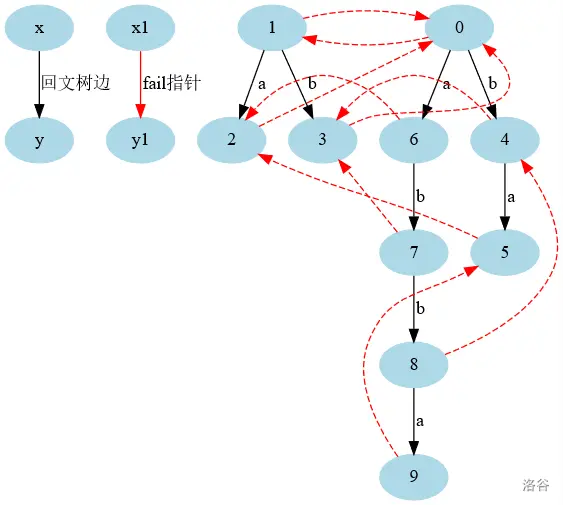
\includegraphics[scale=0.4]{lyh/PAM.png}
%     \caption{PAM}
% \end{figure}
